\section{Methodology}
\label{sec:methods}

\subsection{Problem formulation}

Let $x\in\mathbb{R}^8$ be the parameter vector of a visit and $y=g(x)$ its capped WQI (\cref{eq:wqi}). For a parameter subset $S\subseteq\{1,\dots,8\}$ we learn $f_S:\mathbb{R}^{|S|}\to\mathbb{R}$ minimising squared error on training visits. We evaluate $f_S(x_S)$ against the fixed $y$ on held-out visits. The irreducible error of $f_S$ is the part of $y$ that depends on the unobserved parameters $x_{\bar S}$ and cannot be inferred from $x_S$ through their correlations.

\subsection{Parameter subsets}
\label{sec:methods-subsets}

\Cref{tab:subsets} lists the twelve named subsets. The first four (\sub{S3}, \sub{S5}, \sub{S7}, \sub{Full-8}) were fixed \emph{before} any modelling, from pooled fill rates, in the project methodology. They are kept unchanged so that the original plan can be assessed. The others were added in this study for three reasons: \sub{S4-routine} reflects the panel actually reported every year (\cref{sec:data-availability}); the \sub{I}-subsets follow the importance analysis (\cref{sec:res-importance}); and the \sub{Sensor} subsets contain only parameters measurable instantly with field probes. In addition, all $2^8-1=255$ subsets are evaluated with XGBoost (\cref{sec:res-subsets}).

\begin{table}[h]
\centering\small
\caption{Named parameter subsets. ``Lab'' marks inputs that need laboratory incubation or culturing.}
\label{tab:subsets}
\begin{tabularx}{\textwidth}{llcX}
\toprule
Name & Parameters & $k$ & Rationale \\
\midrule
\sub{S3} & pH, DO, BOD (lab) & 3 & Pre-registered: best-covered parameters \\
\sub{S4-routine} & pH, DO, BOD, fecal coliform (lab) & 4 & Panel actually reported every year \\
\sub{S5} & \sub{S4-routine} + EC & 5 & Pre-registered \\
\sub{S7} & \sub{S5} + total coliform, turbidity & 7 & Pre-registered \\
\sub{Full-8} & all eight & 8 & Ceiling \\
\sub{I3-importance} & pH, BOD, turbidity & 3 & Forward selection, first three \\
\sub{I4-importance} & pH, BOD, turbidity, DO & 4 & Forward selection, first four \\
\sub{I5-importance} & \sub{I4} + nitrate-N & 5 & Forward selection, first five \\
\sub{Sensor-3} & pH, DO, EC & 3 & Probe-only, no laboratory \\
\sub{Sensor-4} & pH, DO, EC, turbidity & 4 & Probe-only, no laboratory \\
\sub{S3+context} & \sub{S3} + latitude, longitude, month & 3+4 & Can location/season stand in for missing parameters? \\
\sub{S4-routine+context} & \sub{S4-routine} + latitude, longitude, month & 4+4 & As above \\
\bottomrule
\end{tabularx}
\end{table}

\subsection{Models}

Eight model families are compared, from no-ML to flexible non-parametric (\cref{tab:models}\iffull; full hyper-parameters in \cref{app:hyper}\fi). Hyper-parameters are fixed \emph{a priori} for every subset and training size. They are not tuned per fold, so that differences between subsets are not confounded with differences in tuning effort. For distance-based and linear models, the six heavy-tailed parameters are transformed with $\log(1+x)$ and all inputs are standardised. Tree models receive raw values.

\begin{table}[h]
\centering\small
\caption{Model families.}
\label{tab:models}
\begin{tabularx}{\textwidth}{lX}
\toprule
Model & Description \\
\midrule
\textbf{Formula} (no ML) & \Cref{eq:wqi} computed from the available parameters only, with weights renormalised over them. This is what a practitioner would do without a model (equivalent to the descriptive \texttt{WQI\_partial}). \\
Linear & Ordinary least squares on log-transformed, standardised inputs. \\
$k$NN & $k=10$ nearest neighbours, distance-weighted. \\
SVR & RBF support-vector regression, $C=30$, $\varepsilon=0.5$. \\
MLP & Two hidden layers (64, 32), L2 $10^{-3}$, early stopping. \\
Random forest & 400 trees, min.\ leaf size 2~\citep{breiman2001}. \\
XGBoost & 600 boosted trees, depth 5, learning rate 0.03, subsampling 0.8~\citep{chen2016}. \\
GPR & Gaussian process, ARD-RBF + white-noise kernel, fitted on at most 1,500 random training rows (subset-of-data approximation)~\citep{rasmussen2006}. \\
\bottomrule
\end{tabularx}
\end{table}

\subsection{Validation schemes}
\label{sec:methods-cv}

The research question is about \emph{data-scarce} systems, i.e.\ places the model has not been trained on. A random split of visits would let a model memorise station identity, since visits from one station are strongly correlated. We therefore use five schemes of increasing difficulty (\cref{fig:cv}):

\begin{enumerate}
  \item \textbf{Random rows} (5-fold): optimistic reference only.
  \item \textbf{Unseen stations} (5-fold grouped by station): \emph{the primary scheme}. Every test station is absent from training, which mimics deploying at a new site. All headline numbers use this scheme.
  \item \textbf{Unseen rivers} (5-fold grouped by river): a whole river is held out.
  \item \textbf{Unseen states} (5-fold grouped by state): regional transfer.
  \item \textbf{Unseen season} (leave-one-season-out: winter, pre-monsoon, monsoon, post-monsoon): the closest available proxy for temporal transfer, since a year-based split is impossible (\cref{sec:data-availability}).
\end{enumerate}

\begin{figure}[t]
  \centering
  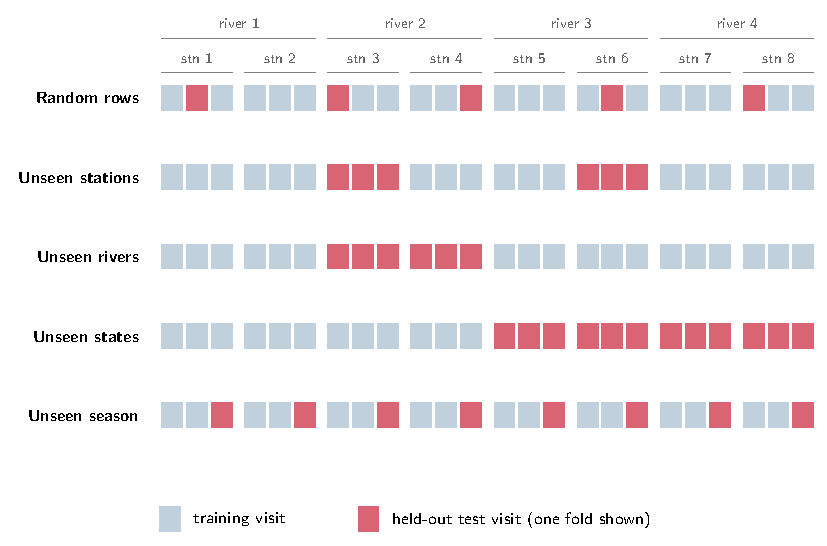
\includegraphics[width=0.8\textwidth]{cv_schemes.pdf}
  \caption{Illustration of the five validation schemes on a toy set of 8 stations on 4 rivers. Red cells are held out in one fold. Only the random-rows scheme lets a test station appear in training.}
  \label{fig:cv}
\end{figure}

Predictions are collected out-of-fold, so every labelled visit is predicted exactly once by a model that never saw it (or its station, river, state or season), and metrics are computed on the pooled predictions. Fold-to-fold standard deviations are reported alongside.

\subsection{Metrics}

On held-out data we report the coefficient of determination \R{} (identical to the Nash--Sutcliffe efficiency, NSE~\citep{nash1970}), RMSE and MAE in WQI points, and KGE~\citep{gupta2009}. We also report \textbf{category accuracy} (exact match among Excellent/Good/Poor/Very Poor), macro-F1 over categories, the share of predictions within $\pm 5$ points, and the share off by two or more categories. For reference, the target's standard deviation is 14.1 points, so RMSE $=14.1$ corresponds to \R{}\,=\,0. A category is 25 points wide.

\subsection{Further experiments}

\paragraph{Importance (\cref{sec:res-importance}).} Spearman correlation, mutual information~\citep{kraskov2004}, random-forest impurity, XGBoost gain, permutation importance on held-out stations, mean absolute SHAP value~\citep{lundberg2017}, drop-column importance (station-CV \R{} lost when a parameter is removed and the model retrained), and the analytic variance share of \cref{sec:wqi-weights}. A consensus rank is the mean of the eight ranks. Greedy forward selection then adds, at each step, the parameter that most increases station-CV \R{}.

\paragraph{Data scarcity (\cref{sec:res-scarcity}).} Inside each station-held-out fold, only a random fraction $\phi\in\{2,5,10,25,50,100\}\%$ of the \emph{training stations} is kept. The test stations stay fixed. Subsampling stations rather than visits reflects how scarcity arises in practice: few monitored sites, not fewer visits per site. Each $\phi<100\%$ is repeated with three random seeds, giving 15 fits per (model, subset, $\phi$).

\paragraph{Uncertainty (\cref{sec:res-uncertainty}).} At a nominal 90\% level we compare (i) Gaussian intervals from the GPR predictive standard deviation, (ii) split-conformal intervals around XGBoost~\citep{vovk2005,barber2021}, whose half-width is the 90\% quantile of absolute residuals from an inner station-grouped CV on the training fold, and (iii) conformalised quantile regression (CQR~\citep{romano2019}) with XGBoost 5\%/95\% quantile models. We report empirical coverage, mean width and coverage by subgroup.

\paragraph{Robustness (\cref{sec:res-robust}).} (A) A single ``universal'' XGBoost trained on copies of the training data with random parameter masking (50\% drop rate, missing values as NaN), compared with a dedicated model per subset. (B) Random missingness of 0--50\% of readings at test time, handled by native NaN support, mean imputation or iterative (MICE-style) imputation. (C) Gaussian measurement noise on test inputs at multiples of typical field error. Absolute noise is used for pH ($\sigma=0.1$) and DO ($\sigma=0.3$\,mg/L), and multiplicative noise for the rest (BOD 15\%, turbidity 10\%, nitrate 15\%, EC 5\%, coliforms 50\%).

\paragraph{Sensitivity (\cref{sec:res-sens}).} The index is recomputed (A) with each standard $S_i$ halved and doubled, plus an EC sweep from 250 to 4,000 \si{\micro S/cm}; (B) with equal weights $W_i=1/8$; and (C) uncapped, predicted on a $\log_{10}$ scale. Key experiments are re-run on each variant.

\paragraph{Deployment (\cref{sec:res-deploy}).} \sub{S3} and \sub{S4-routine} XGBoost models are trained on all 4,861 labelled visits and applied to every river visit with \sub{S3} available but no full panel. Covariate shift is checked with Kolmogorov--Smirnov tests and with adversarial validation: a classifier trained to separate labelled from deployment visits, where an AUC near 0.5 means indistinguishable.

\subsection{Reproducibility}

All experiments are deterministic (seed 42) and are run by the numbered scripts in \texttt{scripts/} (\cref{app:repro}). The software was Python 3.14, pandas 3.0, scikit-learn 1.9, XGBoost 3.4 and SHAP 0.54, on a 16-core CPU. No GPU is needed: the largest experiment takes under an hour.
